\section{Theoretical Analysis}
\label{sec:analysis}

In this section, the circuit depicted in Figure~\ref{circuit} is analysed with two different methods, so as to determine how it behaves, theoretically, both in terms of current in each branch and potential difference between nodes.

To provide for common ground between the theoretical analysis and the simulation run, and to allow for easy comparison, we presented all relevant parameters of the system in three similar tables, in Subsections \ref{sec:mesh}, \ref{sec:node} and \ref{sec:op_point}. The first two were produced using {\bf Octave} and the latter was generated by {\bf Ngspice}.

The $V_n$ stand for the voltage in each node, with respect to the GND node ($V_1=0\;V$). $V_c$, $V_b$, $I_b$ and $I_c$ are represented in the figures. $I_n$ are the currents flowing trough each resistor, in the direction depicted in Figure~\ref{node_fig}, except for $I_6$, as it is, by definition, $I_c$. Lastly, $IV_c$ and $IV_a$ are the currents in each of the voltage sources' branches, with the natural direction (positive to negative).

\subsection{Mesh analysis method}
\label{sec:mesh}

The first method considered is the Mesh analysis method, considering the four meshes present in the circuit. Each mesh is given a label ($\alpha$, $\beta$, $\gamma$ and $\delta$) and an arbitrary direction for the current to flow in, as the below figure shows.

\begin{figure}[H]
  \centering
  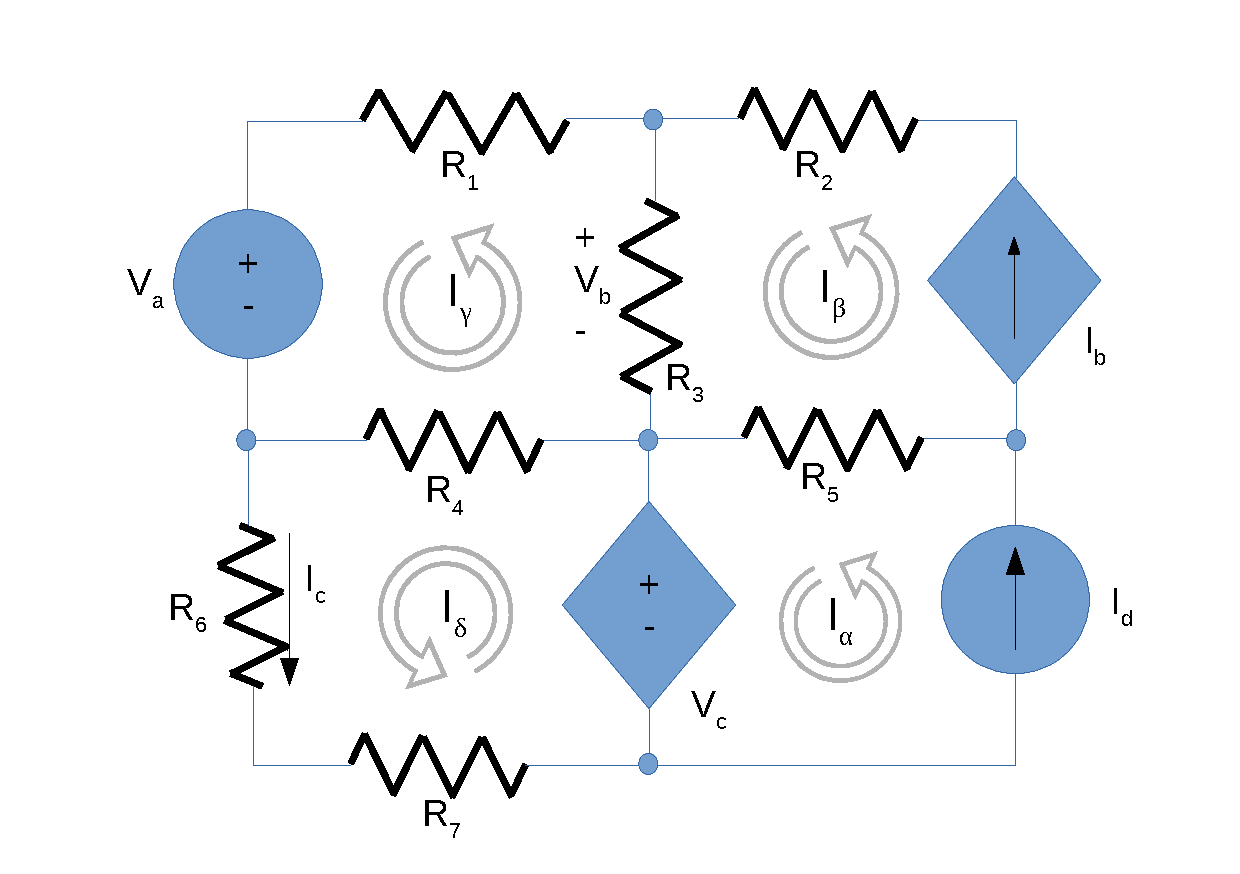
\includegraphics[width=0.5\linewidth]{mesh.pdf}
  \caption{Mesh analysis}
  \label{mesh_fig}
\end{figure}

\newpage

By inspection:

\begin{equation}
  \begin{cases}
    I_{\alpha} = I_d \\
    I_{\beta} = I_b
  \end{cases}
\end{equation}

Applying KVL to the two remaining meshes:

\begin{equation}
  \begin{cases}
    V_a + R_4 (I_\gamma + I_\delta) + R_3 (I_\gamma - I_\beta) + R_1 I_\gamma = 0 \\
    V_c + R_7 I_\delta + R_6 I_\delta + R_4 (I_\delta + I_\gamma) = 0
  \end{cases}
\end{equation}

The conditional sources behave as:

\begin{equation}
  \begin{cases}
  I_b = k_b V_b \\
  V_c = k_c I_c = - k_c I_\delta
  \end{cases}
\end{equation}

Lastly, by Ohm's Law

\begin{equation}
  V_b = R_3 (I_\beta - I_\gamma)
\end{equation}

Manipulating these equations and solving them using {\bf Octave} yields:

%\begin{equation}
%  \begin{bmatrix}
%  1 & 0 & 0 & 0 \\
%  0 & 1-k_b R_3 & k_b R_3 & 0 \\
%  0 & -R_3 & R_1+R_3+R_4 & R_4 \\
%  0 & 0 & R_4 & R_4+R_6+R_7-k_c
%  \end{bmatrix}
%  \begin{bmatrix}
%  I_\alpha \\
%  I_\beta \\
%  I_\gamma \\
%  I_\delta
%  \end{bmatrix}
%  =
%  \begin{bmatrix}
%  I_d \\
%  0 \\
%  -V_a \\
%  0
%  \end{bmatrix}
%\end{equation}

%Solving this system using Octave,

\begin{table}[H]
  \centering
  \begin{tabular}{|c|c|}
    \hline
        {\bf Name} & {\bf Value}\\
        \hline
        \hline
        $I_\alpha\;(A)$ & $0.001000$ \\ 
\hline
$I_\beta\;(A)$ & $-0.000251$ \\ 
\hline
$I_\gamma\;(A)$ & $-0.000240$ \\ 
\hline
$I_\delta\;(A)$ & $-0.000969$ \\ 
\hline
$I_c\;(A)$ & $0.000969$ \\ 
\hline
$I_b\;(A)$ & $-0.000251$ \\ 
\hline
$V_2\;(V)$ & $5.070727$ \\ 
\hline
$V_3\;(V)$ & $4.825468$ \\ 
\hline
$V_4\;(V)$ & $4.304579$ \\ 
\hline
$V_5\;(V)$ & $4.860091$ \\ 
\hline
$V_6\;(V)$ & $8.720760$ \\ 
\hline
$V_7\;(V)$ & $-2.939898$ \\ 
\hline
$V_8\;(V)$ & $-1.950198$ \\ 
\hline
$V_b\;(V)$ & $-0.034623$ \\ 
\hline
$V_c\;(V)$ & $7.799989$ \\ 

        \hline
  \end{tabular}
  \caption{Theoretical results}
  \label{mesh_res}
\end{table}

\newpage

\subsection{Node analysis method}
\label{sec:node}

The second method used was the Node analysis method. With this method, it was possible to determine the voltages in the 8 nodes of the circuit. In Figure~\ref{node_fig}, the directions of the currents chosen to do this analysis are represented, as well as the numerical labels that were given to the nodes.

\begin{figure}[H]
  \centering
  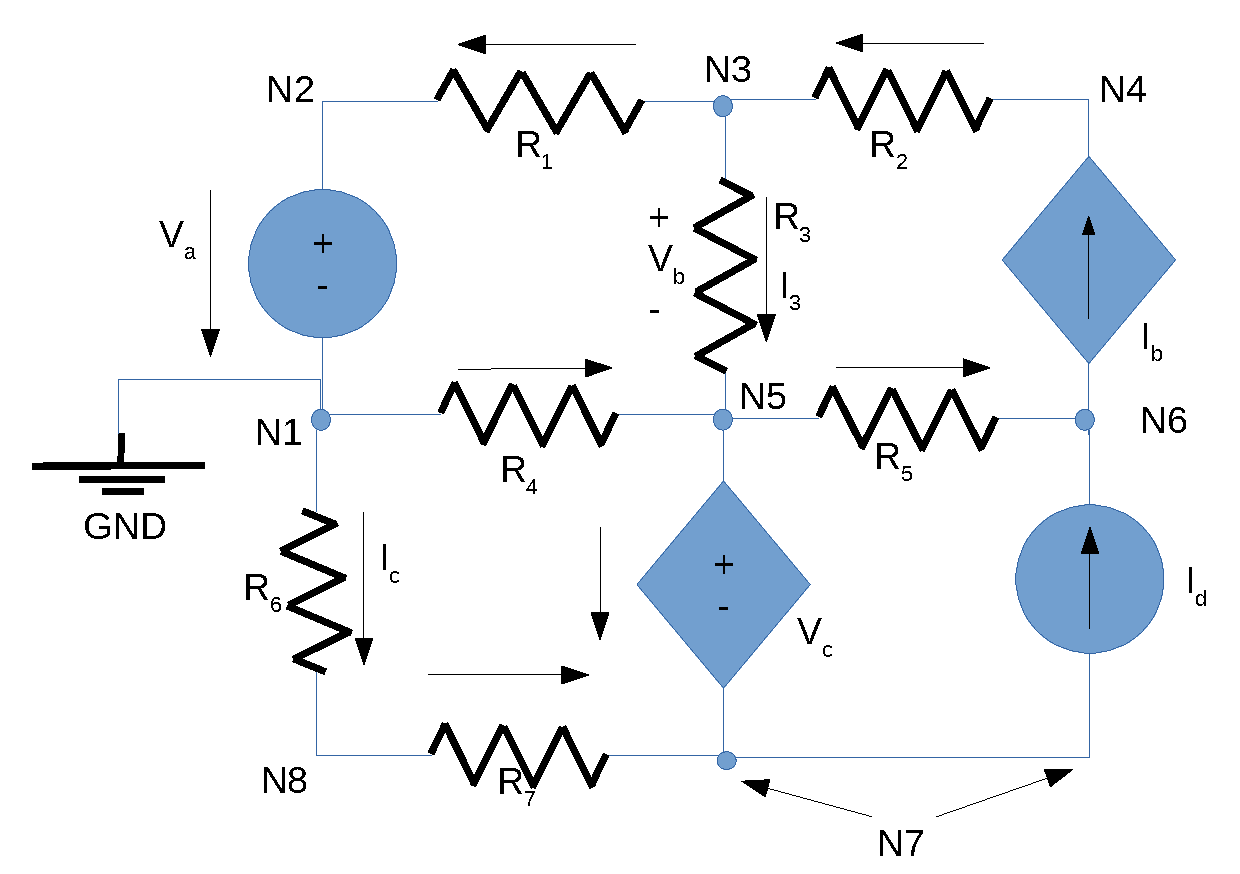
\includegraphics[width=0.5\linewidth]{node.pdf}
  \caption{Node analysis}
  \label{node_fig}
\end{figure}

The node N1 was considered the ground, so:

\begin{equation}
  \begin{cases}
    V_1 = 0 \; V \\
    V_2 = V_a
  \end{cases}
\end{equation}

By applying KCL, it is possible to obtain the following equations:

\begin{equation}
  \begin{cases}
    \frac{V_8}{R_6} + \frac{V_5}{R_4} + \frac{V_3-V_a}{R_1} = 0 \\
    -\frac{V_8}{R_6} - \frac{V_8-V_7}{R_7} = 0 \\
    -\frac{V_3-V_a}{R_1} - \frac{V_3-V_5}{R_3} + \frac{V_4-V_3}{R_2} = 0 \\
    -\frac{V_4-V_3}{R_2} + K_b(V_3-V_5) = 0 \\
    -K_b(V_3-V_5) + \frac{V_5-V_6}{R_5} + I_d = 0
  \end{cases}
\end{equation}

By analysing the dependent voltage source, it is also possible to conclude that

\begin{equation}
  V_5 - V_7 + K_c\frac{V_8}{R_6} = 0
\end{equation}

\newpage

Once again, using {\bf Octave} and the former equations, is possible to determine the voltages in the nodes and the unknown currents and voltages of the circuit:

\begin{table}[H]
  \centering
  \begin{tabular}{|c|c|}
    \hline
        {\bf Name} & {\bf Value} \\
        \hline
        \hline
        $V_2\;(V)$ & $5.070727$ \\ 
\hline
$V_3\;(V)$ & $4.825468$ \\ 
\hline
$V_4\;(V)$ & $4.304579$ \\ 
\hline
$V_5\;(V)$ & $4.860091$ \\ 
\hline
$V_6\;(V)$ & $8.720760$ \\ 
\hline
$V_7\;(V)$ & $-2.939898$ \\ 
\hline
$V_8\;(V)$ & $-1.950198$ \\ 
\hline
$V_b\;(V)$ & $-0.034623$ \\ 
\hline
$I_b\;(V)$ & $-0.000251$ \\ 
\hline
$I_c\;(V)$ & $0.000969$ \\ 
\hline
$V_c\;(V)$ & $7.799989$ \\ 

        \hline
  \end{tabular}
  \caption{Theoretical results}
  \label{node_res}
\end{table} 

The Mesh analysis and the Node analysis are equivalent so, as expected, they produced the same results.


